\textbf{Цель работы:} Исследовать зависимость фототока от величины задерживающего потенциала и частоты падающего излучения, что позволяет вычислить величину постоянной Планка.
             
\section{Теоретическое введение}
    Фотоэффект -- явление испускания электронов фотокатодом, облучаемым светом,  Это явление хорошо объясняется фотонной теорией света. Взаимодействие монохроматического света с веществом можно описывать как взаимодействие с веществом частиц, называемых фотонами, которые обладают энергией $\hbar \omega$ и импульсом $\hbar \omega /c$. При столкновении фотона с электроном фотокатода энергия фотона полностью передается электрону, и фотон прекращает свое существование. Энергетический баланс этого взаимодействия для вылетающих электронов
	описывается уравнением
	\begin{equation}
        \label{energy balance}
	    \hbar \omega = E_{max} + W
	\end{equation}

    \begin{figure}[h!]
        \centering
        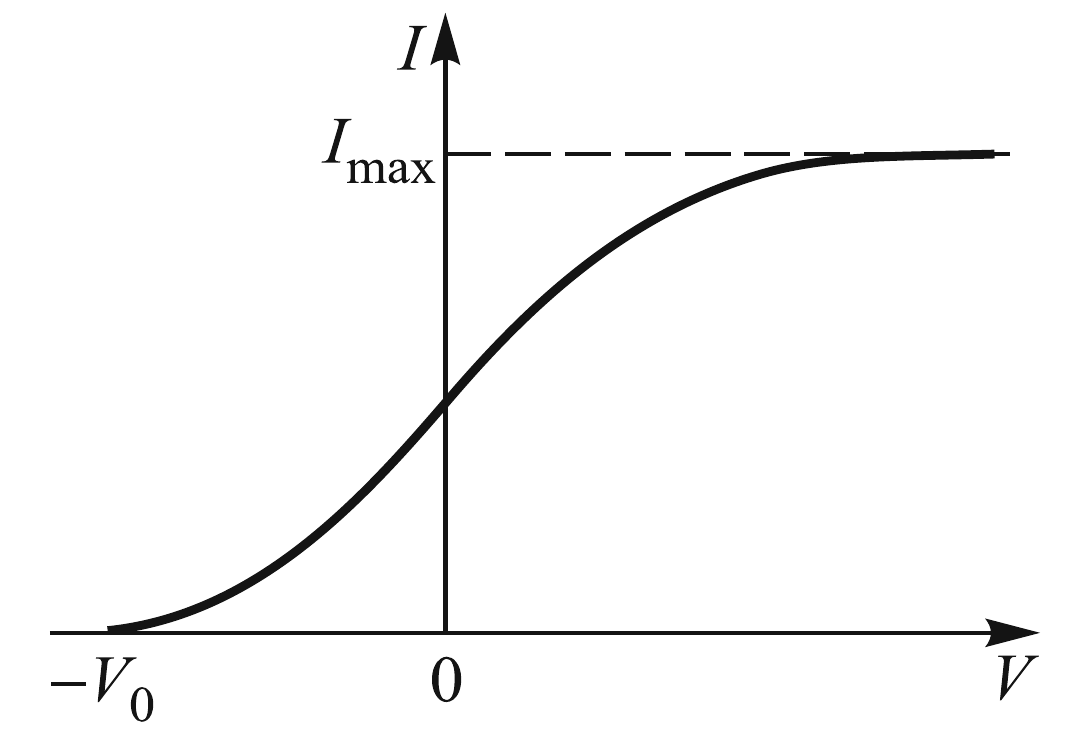
\includegraphics[width = 8.2 cm]{images/I_V_th}
        \caption{Зависимость фототока от напряжения на аноде фотоэлемента}
        \label{pict I(V)}
    \end{figure}
    
	Здесь $E_{max}$ -- максимальная кинетическая энергия электрона после выхода из фотокатода, $W$ -- работа выхода электрона из катода. Реально энергетический спектр вылетевших из фотокатода электронов непрерывен -- он простирается от нуля до $E_{max}$. 
	
	Для измерения энергии вылетевших фотоэлектронов вблизи фотокатода обычно располагается второй электрод (анод), на который подается задерживающий ($V < 0$) или ускоряющий ($V > 0$) потенциал. При достаточно больших ускоряющих напряжениях фототок достигает насыщения (рис. \ref{pict I(V)}): все испущенные электроны попадают на анод.
	
	При задерживающих потенциалах на анод попадают лишь электроны, обладающие достаточно большой кинетической энергией, в то время
	как медленно движущиеся электроны заворачиваются полем и возвращаются на катод. При некотором значении $V = -V_0$ (потенциал запирания) даже наиболее быстрые фотоэлектроны не могут достичь анода.
	Максимальная кинетическая энергия $ E_{max} $ электронов связана с запирающим потенциалом $V_0$ очевидным соотношением $E_{max} = eV_0$. Тогда \eqref{energy balance} примет вид, называемый уравнением Эйнштейна:
	
	\begin{equation}
        \label{Einsteain}
	    eV_0 = \hbar\omega - W 
	\end{equation}
	
	Чтобы определить величину запирающего напряжения, нам надо правильно экстраполировать получаемую токовую зависимость к нулю, т. е. определить, какова функциональная зависимость $I(V)$. Расчет для простейшей геометрии -- плоский катод, освещаемый светом, и параллельный ему анод -- приводит к зависимости
	
	\begin{equation}
        \label{sqrt I = V}
	    \sqrt{I} \propto V_0 - V,
	\end{equation}
	т. е. корень квадратный из фототока линейно зависит от запирающего напряжения. Эта зависимость хорошо описывает экспериментальные данные.
	
	В работе изучается зависимость фототока из фотоэлемента от величины задерживающего потенциала $V$ для различных частот света $\omega$, лежащих в видимой области спектра. С целью экспериментальной проверки уравнения Эйнштейна определяются потенциалы запирания
	$V_0$ при разных частотах света и строится зависимость $ V_0(\omega) $, которая, как это следует из \eqref{Einsteain}, должна иметь вид
	
	\begin{equation}
        \label{V(w)}
	    V_0 (\omega) = \dfrac{\hbar\omega - W}{e}
	\end{equation}

    \begin{figure}[h!]
        \centering
        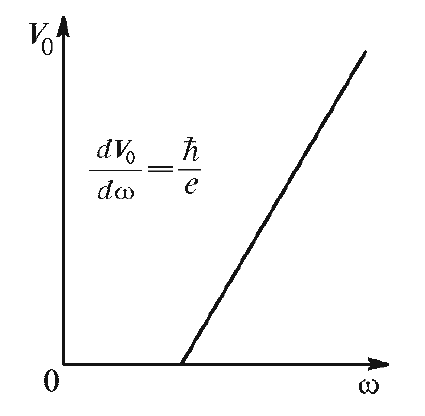
\includegraphics[width = 6.8 cm]{images/V_omega_th}
        \caption{Зависимость запирающего потенциала от частоты света}
        \label{pict V(w)}
    \end{figure}
	
	Потенциал запирания $V_0$ для любого катода линейно зависит от частоты света $\omega$. По наклону прямой на графике $V_0(\omega)$ (рис. \ref{pict V(w)}) можно определить постоянную Планка:
	
	\begin{equation}
        \label{dV/dw}
	    \dfrac{dV_0}{d\omega} = \dfrac{\hbar}{e}
	\end{equation}
	
	Как показывает формула \eqref{dV/dw}, угол наклона прямой $V_0(\omega) $ не зависит от рода вещества, из которого изготовлен фотокатод. От рода вещества, однако, зависит величина фототока, работа выхода $W$ и форма кривой $I(V)$ (рис. \ref{pict I(V)}). Все это определяет выбор пригодных для опыта катодов.

\section{Экспериментальная установка}

    \begin{figure}[h!]
        \centering
        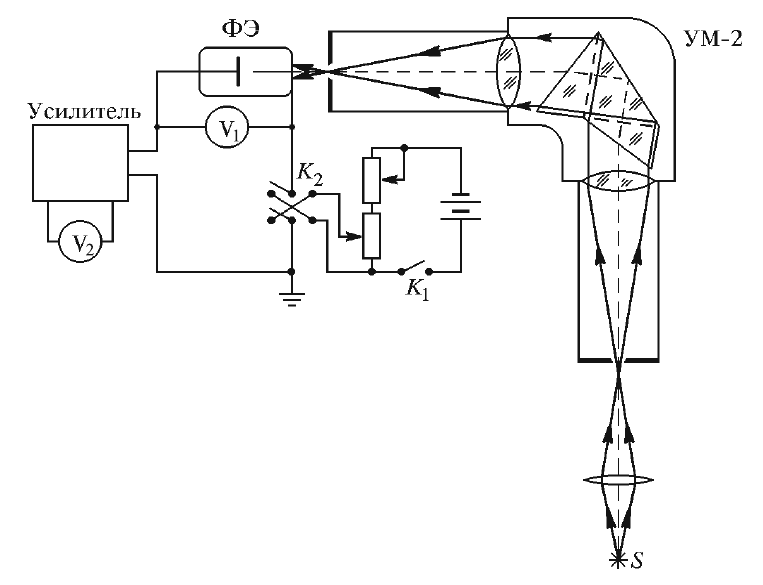
\includegraphics[width = 12 cm]{images/exp_scheme}
        \caption{Принципиальная схема экспериментальной установки}
        \label{exp_scheme}
    \end{figure}

    Свет от источника $S$ (обычная электрическая лампа накаливания) с помощью конденсора фокусируется на входную щель призменного монохроматора УМ-2, выделяющего узкий спектральный интервал, и попадает на катод фотоэлемента ФЭ.

    Фотоэлемент конструктивно представляет собой откачанный до высокого вакуума стеклянный баллон диаметром 25 мм и высотой 30 мм. Внутри баллона расположены два электрода: фотокатод и анод. Фотокатод представляет собой тонкую пленку металла, легированного элементами $Na$, $K$, $Sb$ и $Cs$ и расположенного на массивной металлической пластине. Анод фотоэлемента выполнен в виде пояска тонкой пленки, осажденной на внутренней части боковой поверхности вверху баллона. Такое расположение фотокатода и анода обеспечивает наиболее полный сбор на аноде электронов, эмитированных фотокатодом. Фотокатод и анод имеют вплавленные в стекло колбы никелевые выводы для подключения к внешней схеме. Такой фотоэлемент обладает спектральной чувствительностью в области длин волн от 300 до
    850 нм. Наибольшая чувствительность ФЭ лежит в области от 400 до 500 нм.

    Фототок, протекающий в фотоэлементе, мал, особенно при потенциалах $V$, близких к $V_0$ , и не может быть измерен непосредственно. Для его измерения используется усилитель постоянного тока. Для уменьшения погрешностей измерений, обусловленных наводками, усилитель ототока смонтирован в одном корпусе с ФЭ. Абсолютные значения ототока нам не нужны, поэтому он измеряется в относительных единицах цировым вольтметром $V_2$ , подключенным к выходу усилителя. Эти показания пропорциональны величине измеряемого тока. Тормозящий потенциал регулируется при помощи двух потенциометров "Грубо" и "Плавно", установленных на корпусе блока питания установки. Измерение тормозящего потенциала осуществляется
    с помощью цирового вольтметра $V_1$.

    Контактная разность потенциалов между катодом и анодом мешает точному определению величины $V_0$ , но не оказывает влияния на определение постоянной Планка, которая выражается через производную $dV_0 / d\omega$.
    
\section{Ход работы}

    \begin{enumerate}
        \item Выполним градуировку монохроматора.
        \begin{table}[H]
            \centering
            \begin{tabular}{|c|c|c|c|c|c|}
                \hline
                $\lambda$ & $\theta$ & $\lambda$ & $\theta$ & $\lambda$ & $\theta$ \\ \hline
                540.1     & 1840     & 609.6     & 2218     & 633.4     & 2318     \\ \hline
                585.2     & 2102     & 614.3     & 2238     & 638.2     & 2336     \\ \hline
                588.2     & 2118     & 616.3     & 2248     & 640.2     & 2342     \\ \hline
                594.5     & 2148     & 621.7     & 2268     & 650.6     & 2380     \\ \hline
                597.6     & 2162     & 626.6     & 2288     & 653.2     & 2388     \\ \hline
                603.0     & 2183     & 630.4     & 2302     & 659.8     & 2416     \\ \hline
                607.4     & 2207     & --        & --       & --        & --       \\ \hline
                \end{tabular}
            \caption{Калибровочные данные монохроматора}
        \end{table}

        \begin{figure}[H]
            \centering
            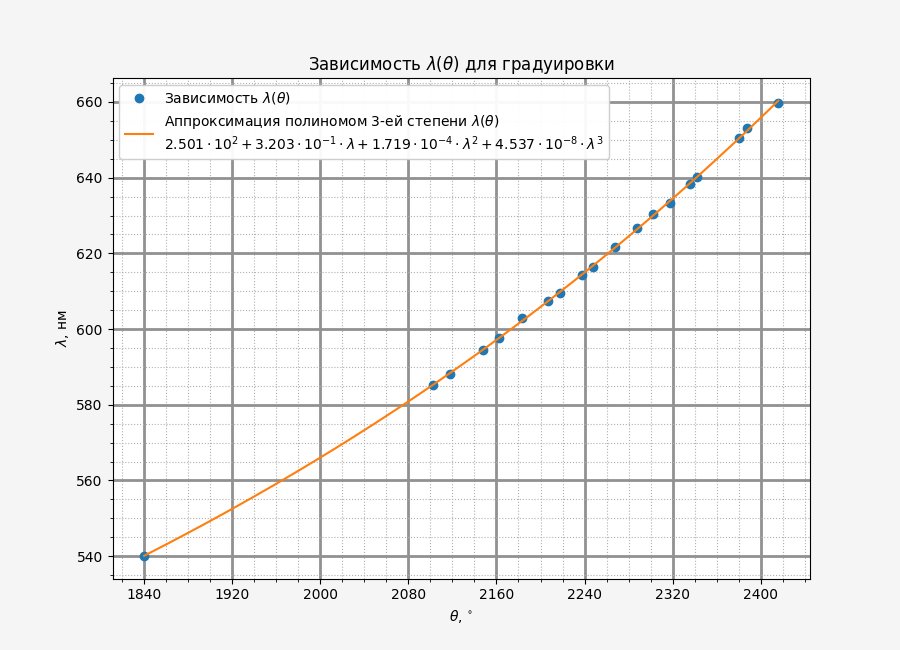
\includegraphics[width = 14.5 cm]{images/calibration}
            \caption{Калибровочные кривая монохроматора}
            \label{calibr}
        \end{figure}

        Заметим, что среднеквартичное отклонение измеренныз величин и величин модели равно $\sigma_{\lambda} = 0.15$ нм, поэтому модель можно считать точной.

        \item Снимем зависимость $V_1(V)$, затем построим графики $\sqrt{(V_1)}(V)$, определим соответствующие пороговые значения напряжений $V_0$.
        
        \begin{table}[H]
            \centering
            \begin{tabular}{|ccc|ccc|ccc|}
                \hline
                \multicolumn{3}{|c|}{$\lambda = 540.1$, нм}                                                     & \multicolumn{3}{c|}{$\lambda = 582.8$, нм}                                                     & \multicolumn{3}{c|}{$\lambda = 617.3$, нм}                                                     \\ \hline
                \multicolumn{1}{|c|}{$V$, В} & \multicolumn{1}{c|}{$V_1$, В} & $\sqrt{(V_1)}$, $\text{В}^{1/2}$ & \multicolumn{1}{c|}{$V$, В} & \multicolumn{1}{c|}{$V_1$, В} & $\sqrt{(V_1)}$, $\text{В}^{1/2}$ & \multicolumn{1}{c|}{$V$, В} & \multicolumn{1}{c|}{$V_1$, В} & $\sqrt{(V_1)}$, $\text{В}^{1/2}$ \\ \hline
                \multicolumn{1}{|c|}{-0.70}  & \multicolumn{1}{c|}{0.01}     & 0.10                             & \multicolumn{1}{c|}{-0.62}  & \multicolumn{1}{c|}{0.01}     & 0.10                             & \multicolumn{1}{c|}{-0.43}  & \multicolumn{1}{c|}{0.01}     & 0.10                             \\ \hline
                \multicolumn{1}{|c|}{-0.62}  & \multicolumn{1}{c|}{0.03}     & 0.17                             & \multicolumn{1}{c|}{-0.58}  & \multicolumn{1}{c|}{0.02}     & 0.14                             & \multicolumn{1}{c|}{-0.38}  & \multicolumn{1}{c|}{0.02}     & 0.14                             \\ \hline
                \multicolumn{1}{|c|}{-0.54}  & \multicolumn{1}{c|}{0.04}     & 0.20                             & \multicolumn{1}{c|}{-0.56}  & \multicolumn{1}{c|}{0.02}     & 0.14                             & \multicolumn{1}{c|}{-0.32}  & \multicolumn{1}{c|}{0.04}     & 0.20                             \\ \hline
                \multicolumn{1}{|c|}{-0.47}  & \multicolumn{1}{c|}{0.07}     & 0.26                             & \multicolumn{1}{c|}{-0.46}  & \multicolumn{1}{c|}{0.05}     & 0.22                             & \multicolumn{1}{c|}{-0.25}  & \multicolumn{1}{c|}{0.08}     & 0.28                             \\ \hline
                \multicolumn{1}{|c|}{-0.37}  & \multicolumn{1}{c|}{0.11}     & 0.33                             & \multicolumn{1}{c|}{-0.39}  & \multicolumn{1}{c|}{0.08}     & 0.28                             & \multicolumn{1}{c|}{-0.20}  & \multicolumn{1}{c|}{0.10}     & 0.32                             \\ \hline
                \multicolumn{1}{|c|}{-0.26}  & \multicolumn{1}{c|}{0.15}     & 0.39                             & \multicolumn{1}{c|}{-0.33}  & \multicolumn{1}{c|}{0.10}     & 0.32                             & \multicolumn{1}{c|}{-0.10}  & \multicolumn{1}{c|}{0.15}     & 0.39                             \\ \hline
                \multicolumn{1}{|c|}{-0.13}  & \multicolumn{1}{c|}{0.21}     & 0.46                             & \multicolumn{1}{c|}{-0.21}  & \multicolumn{1}{c|}{0.16}     & 0.40                             & \multicolumn{1}{c|}{-0.01}  & \multicolumn{1}{c|}{0.20}     & 0.45                             \\ \hline
                \multicolumn{1}{|c|}{0.02}   & \multicolumn{1}{c|}{0.29}     & 0.54                             & \multicolumn{1}{c|}{-0.11}  & \multicolumn{1}{c|}{0.20}     & 0.45                             & \multicolumn{1}{c|}{0.03}   & \multicolumn{1}{c|}{0.22}     & 0.47                             \\ \hline
                \multicolumn{1}{|c|}{0.16}   & \multicolumn{1}{c|}{0.36}     & 0.60                             & \multicolumn{1}{c|}{0.00}   & \multicolumn{1}{c|}{0.26}     & 0.51                             & \multicolumn{1}{c|}{0.11}   & \multicolumn{1}{c|}{0.27}     & 0.52                             \\ \hline
                \multicolumn{1}{|c|}{0.28}   & \multicolumn{1}{c|}{0.40}     & 0.63                             & \multicolumn{1}{c|}{0.12}   & \multicolumn{1}{c|}{0.32}     & 0.57                             & \multicolumn{1}{c|}{0.19}   & \multicolumn{1}{c|}{0.34}     & 0.58                             \\ \hline
                \multicolumn{1}{|c|}{0.38}   & \multicolumn{1}{c|}{0.42}     & 0.65                             & \multicolumn{1}{c|}{0.29}   & \multicolumn{1}{c|}{0.39}     & 0.62                             & \multicolumn{1}{c|}{0.32}   & \multicolumn{1}{c|}{0.39}     & 0.62                             \\ \hline
                \multicolumn{1}{|c|}{0.44}   & \multicolumn{1}{c|}{0.44}     & 0.66                             & \multicolumn{1}{c|}{0.39}   & \multicolumn{1}{c|}{0.43}     & 0.66                             & \multicolumn{1}{c|}{0.41}   & \multicolumn{1}{c|}{0.42}     & 0.65                             \\ \hline
                \multicolumn{1}{|c|}{0.51}   & \multicolumn{1}{c|}{0.45}     & 0.67                             & \multicolumn{1}{c|}{0.51}   & \multicolumn{1}{c|}{0.44}     & 0.66                             & \multicolumn{1}{c|}{0.52}   & \multicolumn{1}{c|}{0.44}     & 0.66                             \\ \hline
            \end{tabular}
            \caption{Данные зависимостей $\sqrt{(V_1)}(V)$}
        \end{table}

        \begin{table}[H]
            \centering
            \begin{tabular}{|ccc|ccc|}
                \hline
                \multicolumn{3}{|c|}{$\lambda = 639.6$, нм}                                                     & \multicolumn{3}{c|}{$\lambda = 668.7$, нм}                                                     \\ \hline
                \multicolumn{1}{|c|}{$V$, В} & \multicolumn{1}{c|}{$V_1$, В} & $\sqrt{(V_1)}$, $\text{В}^{1/2}$ & \multicolumn{1}{c|}{$V$, В} & \multicolumn{1}{c|}{$V_1$, В} & $\sqrt{(V_1)}$, $\text{В}^{1/2}$ \\ \hline
                \multicolumn{1}{|c|}{-0.30}  & \multicolumn{1}{c|}{0.02}     & 0.14                             & \multicolumn{1}{c|}{-0.16}  & \multicolumn{1}{c|}{0.04}     & 0.20                             \\ \hline
                \multicolumn{1}{|c|}{-0.19}  & \multicolumn{1}{c|}{0.06}     & 0.24                             & \multicolumn{1}{c|}{-0.05}  & \multicolumn{1}{c|}{0.09}     & 0.30                             \\ \hline
                \multicolumn{1}{|c|}{-0.12}  & \multicolumn{1}{c|}{0.10}     & 0.32                             & \multicolumn{1}{c|}{0.00}   & \multicolumn{1}{c|}{0.12}     & 0.35                             \\ \hline
                \multicolumn{1}{|c|}{-0.03}  & \multicolumn{1}{c|}{0.15}     & 0.39                             & \multicolumn{1}{c|}{0.09}   & \multicolumn{1}{c|}{0.16}     & 0.40                             \\ \hline
                \multicolumn{1}{|c|}{0.02}   & \multicolumn{1}{c|}{0.18}     & 0.42                             & \multicolumn{1}{c|}{0.13}   & \multicolumn{1}{c|}{0.19}     & 0.44                             \\ \hline
                \multicolumn{1}{|c|}{0.09}   & \multicolumn{1}{c|}{0.22}     & 0.47                             & \multicolumn{1}{c|}{0.17}   & \multicolumn{1}{c|}{0.22}     & 0.47                             \\ \hline
                \multicolumn{1}{|c|}{0.14}   & \multicolumn{1}{c|}{0.26}     & 0.51                             & \multicolumn{1}{c|}{0.22}   & \multicolumn{1}{c|}{0.26}     & 0.51                             \\ \hline
                \multicolumn{1}{|c|}{0.23}   & \multicolumn{1}{c|}{0.32}     & 0.57                             & \multicolumn{1}{c|}{0.30}   & \multicolumn{1}{c|}{0.32}     & 0.57                             \\ \hline
                \multicolumn{1}{|c|}{0.31}   & \multicolumn{1}{c|}{0.36}     & 0.60                             & \multicolumn{1}{c|}{0.36}   & \multicolumn{1}{c|}{0.35}     & 0.59                             \\ \hline
                \multicolumn{1}{|c|}{0.39}   & \multicolumn{1}{c|}{0.40}     & 0.63                             & \multicolumn{1}{c|}{0.41}   & \multicolumn{1}{c|}{0.38}     & 0.62                             \\ \hline
                \multicolumn{1}{|c|}{0.48}   & \multicolumn{1}{c|}{0.43}     & 0.66                             & \multicolumn{1}{c|}{0.45}   & \multicolumn{1}{c|}{0.41}     & 0.64                             \\ \hline
                \multicolumn{1}{|c|}{0.54}   & \multicolumn{1}{c|}{0.45}     & 0.67                             & \multicolumn{1}{c|}{0.50}   & \multicolumn{1}{c|}{0.50}     & 0.71                             \\ \hline
            \end{tabular}
            \caption{Данные зависимостей $\sqrt{(V_1)}(V)$}
        \end{table}

        \begin{figure}[H]
            \centering
            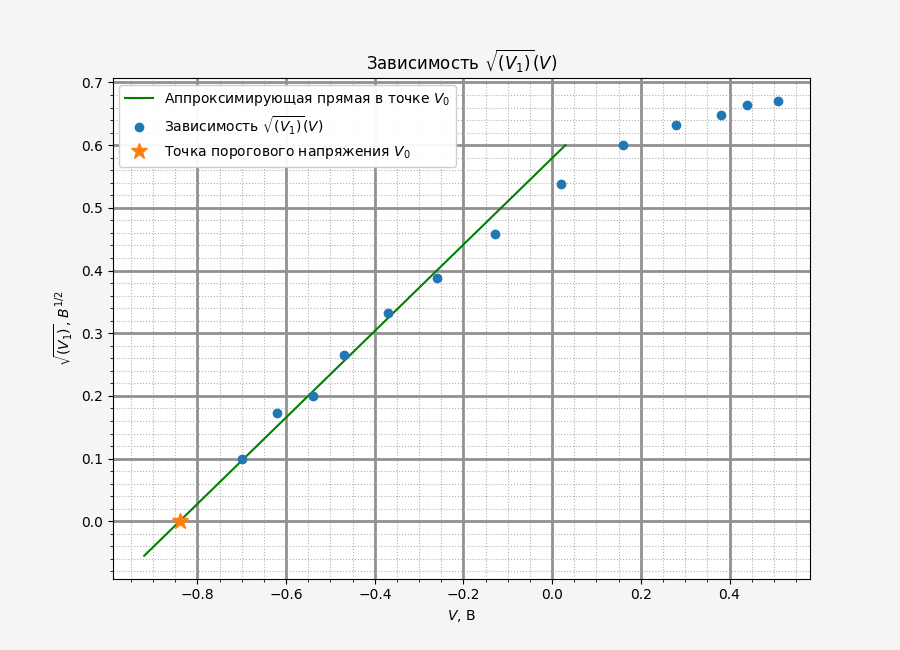
\includegraphics[width = 12 cm]{images/plot_1}
            \caption{Зависимость $\sqrt{(V_1)}(V)$ для $\lambda = 540.1$, нм}
            \label{V_V1_1}
        \end{figure}

        \begin{figure}[H]
            \centering
            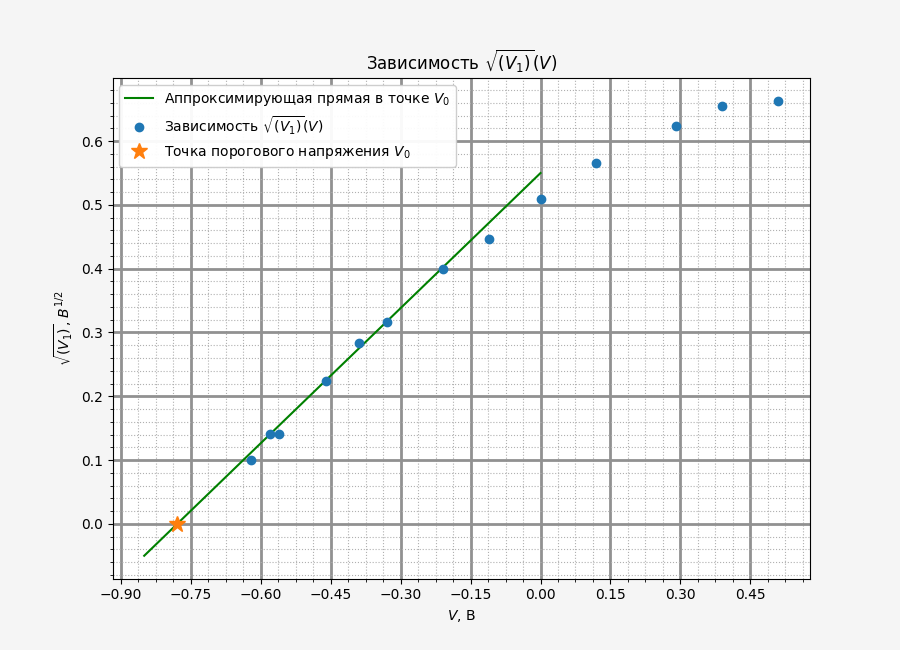
\includegraphics[width = 12 cm]{images/plot_2}
            \caption{Зависимость $\sqrt{(V_1)}(V)$ для $\lambda = 582.8$, нм}
            \label{V_V1_2}
        \end{figure}

        \begin{figure}[H]
            \centering
            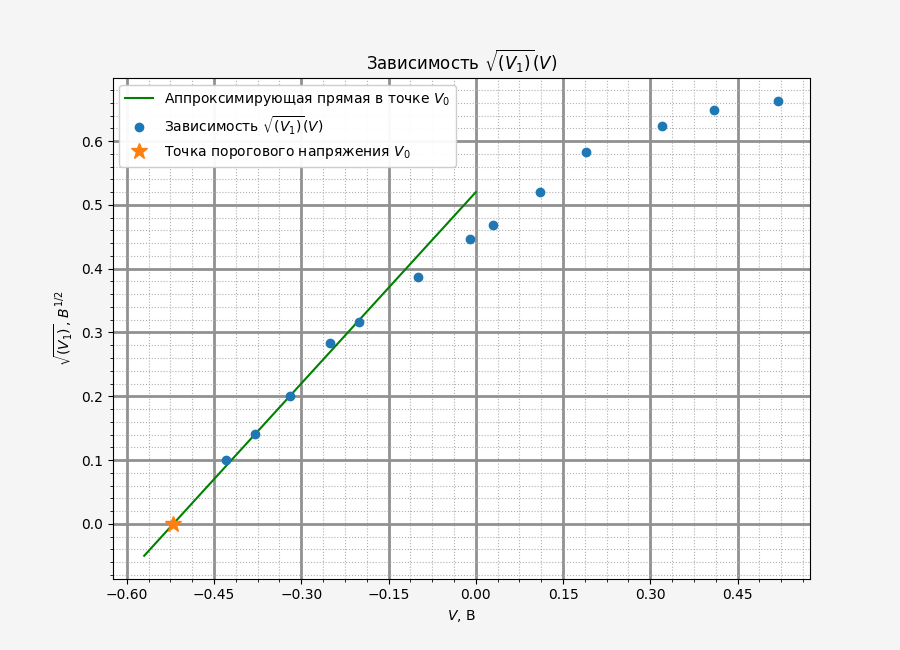
\includegraphics[width = 12 cm]{images/plot_3}
            \caption{Зависимость $\sqrt{(V_1)}(V)$ для $\lambda = 617.3$, нм}
            \label{V_V1_3}
        \end{figure}

        \begin{figure}[H]
            \centering
            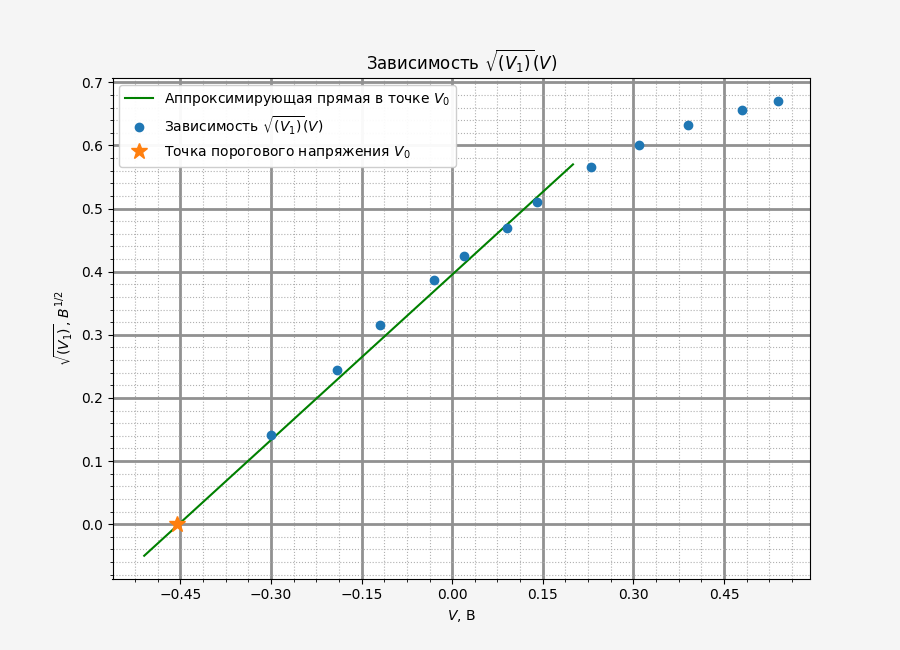
\includegraphics[width = 12 cm]{images/plot_4}
            \caption{Зависимость $\sqrt{(V_1)}(V)$ для $\lambda = 639.6$, нм}
            \label{V_V1_4}
        \end{figure}

        \begin{figure}[H]
            \centering
            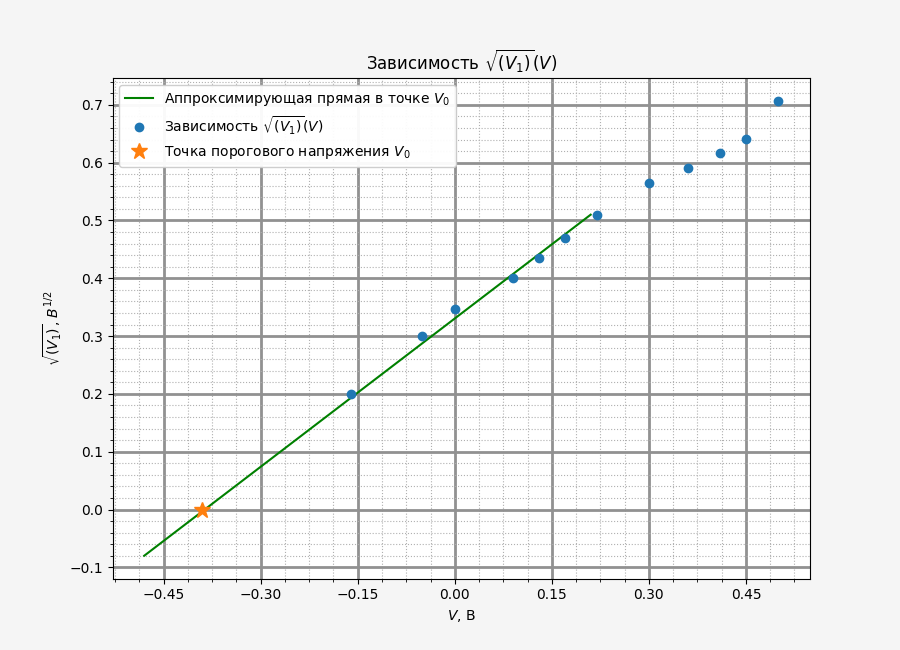
\includegraphics[width = 12 cm]{images/plot_5}
            \caption{Зависимость $\sqrt{(V_1)}(V)$ для $\lambda = 668.7$, нм}
            \label{V_V1_5}
        \end{figure}

        \item Построим таблицу и график зависимости $V_0(\omega)$
        
        \begin{table}[H]
            \centering
            \begin{tabular}{|c|c|c|}
            \hline
            $V_0$, В & \multicolumn{1}{l|}{$\lambda$, нм} & \multicolumn{1}{l|}{$\omega \cdot 10^{15}$, $\text{с}^{-1}$} \\ \hline
            -0.842   & 540.1                              & 3.488                                                        \\ \hline
            -0.781   & 582.8                              & 3.232                                                        \\ \hline
            -0.521   & 617.3                              & 3.051                                                        \\ \hline
            -0.455   & 639.6                              & 2.945                                                        \\ \hline
            -0.391   & 668.7                              & 2.817                                                        \\ \hline
            \end{tabular}
            \caption{Таблица зависимости $V_0(\omega)$}.
        \end{table}

        \begin{figure}[H]
            \centering
            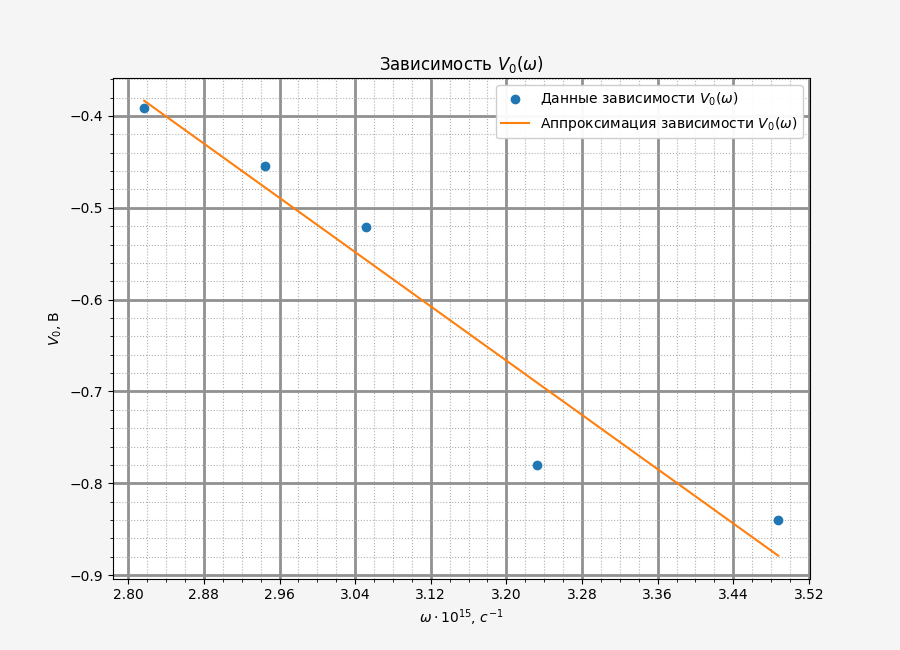
\includegraphics[width = 14.5 cm]{images/V_omega}
            \caption{График зависимости $V_0(\omega)$}
        \end{figure}

        С помощью МНК найдём значение коэффициента наклона графика:
        \begin{equation}
            \Bigg| \frac{dV_0}{d\omega} \Bigg| = (0.719 \pm 0.127) \cdot 10^{-15} \; \text{В} \cdot \text{с} \Rightarrow \hbar = (1.115 \pm 0.203) \cdot 10^{-34} \; \text{Дж} \cdot \text{с}
        \end{equation}

        Таким образом, полученное значение постоянной Дирака совпадает с теоретическим значением $\hbar = 1.054 \cdot 10^{-34} \; \text{Дж} \cdot \text{с}$.
        
    \end{enumerate}

\section{Заключение}

    В результате работы подверждена квантовая теория света и получено значением постоянной Дирака $\hbar = (1.115 \pm 0.203) \cdot 10^{-34} \; \text{Дж} \cdot \text{с}$, которое совпадает с теортическим значением $\hbar = 1.054 \cdot 10^{-34} \; \text{Дж} \cdot \text{с}$.